\section{Lecture 4. Problems with Perfect State Information}
\subsection{Linear System and Quadratic Cost}
Definition
\begin{itemize}
    \item State: $x_k\in \mathbb{R}^{n\times 1}$
    \item Control: $u_k\in\mathbb{R}^{m\times 1}$
    \item Disturbance: $w_k\in\mathbb{R}^{n\times 1}$
    \begin{itemize}
        \item independent and zero mean $\mathbb{E}(w_k)=0$
    \end{itemize}
    \item Linear Dynamics: $x_{k+1}=A_kx_k+B_ku_k+w_k$
    \begin{itemize}
        \item $A_k \in \mathbb{R}^{n\times n}$, $B_k\in\mathbb{R}^{n\times m}$
    \end{itemize}
    \item Quadratic Stage Cost: $u_k^T R_k u_k+x_k^TQ_kx_k$
    \begin{itemize}
        \item $R_k\in\mathbb{R}^{m\times m}$ positive definite symmetric matrix
        \item $Q_k\in\mathbb{R}^{n\times n}$ positive semidefinite symmetric matrix
    \end{itemize}
    \item Terminal Cost: $J_N(x_N)=x_N^TQ_Nx_N$
\end{itemize}

\subsection{Derivation}
DP algorithm
\begin{itemize}
    \item $J_N(x_N)=x_N^TQ_Nx_N$
    \item $J_k(x_k)=\min_{u_k}\mathbb{E}\{ x_k^TQ_kx_k + u_k^TR_ku_k + J_{k+1}(A_kx_k+B_ku_k+w_k) \}$
    \item $J_{N-1}(x_{N-1})=\min_{u_{N-1}} \{ x_{N-1}^TQ_{N-1}x_{N-1} + u_{N-1}^TR_{N-1}u_{N-1} + (A_{N-1}x_{N-1}+B_{N-1}u_{N-1}+w_{N-1})^TQ_N(A_{N-1}x_{N-1}+B_{N-1}u_{N-1}+w_{N-1}) \}$
    \item $(A_{N-1}x_{N-1}+B_{N-1}u_{N-1}+w_{N-1})^TQ_N(A_{N-1}x_{N-1}+B_{N-1}u_{N-1}+w_{N-1})$ \\
    $ = x_{N-1}^TA_{N-1}^TQ_NA_{N-1}x_{N-1} + u_{N-1}^TB_{N-1}^TQ_NB_{N-1}u_{N-1} + \mathbb{E}(w_{N-1}^TQ_Nw_{N-1}) + 2x_{N-1}^TA_{N-1}^TQ_NB_{N-1}u_{N-1}$ \\
    \item Define
    \begin{itemize}
        \item $C = \underbrace{R_{N-1}}_{>0} + \underbrace{B_{N-1}^T Q_N B_{N-1}}_{\geq 0} >0$ (invertible), and $C\in\mathbb{R}^{m\times m}$
        \item $D = x_{N-1}^TA_{N-1}^TQ_N B_{N-1}$, and $D\in\mathbb{R}^{1\times m}$
        \item $E = x_{N-1}^TQ_{N-1}x_{N-1} + x_{N-1}^TA_{N-1}^TQ_NA_{N-1}x_{N-1} + w_{N-1}^TQ_Nw_{N-1}$ independent of $u_{N-1}$, and $E\in\mathbb{R}$
    \end{itemize}
    \item $J_{N-1}(x_{N-1})=\min_{u_{N-1}} \{ u_{N-1}^T C u_{N-1} + 2Du_{N-1} + E\} $
    \item Since $J_{N-1}(x_{N-1})$ is quadratic in $u_{N-1}$, so $Cu_{N-1}^*=-D^T$ and $u_{N-1}^*=-C^{-1}D^T$
    \item $u_{N-1}^* = -(R_{N-1}+B_{N-1}^T Q_N B_{N-1})^{-1} B_{N-1}^T Q_N A_{N-1} \cdot x_{N-1}$ (Linear in state $x_{N-1}$)
    \item $J_{N-1}(x_{N-1}) = x_{N-1}^TK_{N-1}x_{N-1} + w_{N-1}^TQ_Nw_{N-1}$ \\
    where $K_{N-1}=A_{N-1}^T(Q_N-Q_NB_{N-1}(B_{N-1}^TQ_NB_{N-1}+R_{N-1})^{-1}B_{N-1}^TQ_N)A_{N-1}+Q_{N-1}$ \\
    and $K_{N-1}$ is symmetric positive semidefinite
    \item $J_{N-2}(x_{N-2})=\min_{u_{N-2}} \{ x_{N-2}^TQ_{N-2}x_{N-2} + u_{N-2}^TR_{N-2}u_{N-2} + (A_{N-2}x_{N-2}+B_{N-2}u_{N-2}+w_{N-2})^TK_{N-1}(A_{N-2}x_{N-2}+B_{N-2}u_{N-2}+w_{N-2}) \}$
\end{itemize}

Conclusion
\begin{itemize}
    \item Optimal policy: $u^*=L_kx_k$
    \item Optimal cost: $J_k(x_k)=x_k^TK_kx_k+\text{\rm constant}$\\
    where $L_k=-(B_k^TK_{k+1}B_k+R_k)^{-1}B_k^TK_{k+1}A_k$\\
    and $K_k$ are symmetric positive semidefinite matrices given by 
    \[K_N = Q_N\]
    \[K_k = A_k^T(K_{k+1}-K_{k+1}B_k(B_k^TK_{k+1}B_k+R_k)^{-1}B_k^TK_{k+1})A_k+Q_k\]

    \item This is called the \emph{discrete-time Riccati equation}
    \item Certainty equivalence holds \\ optimal policy is the same as when $w_k$ is replaced by $\mathbb{E}\{ w_k \}=0$ 
\end{itemize}

\subsection{Asymptotic Behavior of Riccati Equation}
What if finite horizon $\to$ infinite horizon ($N\to\infty$)?
\begin{itemize}
    \item $u^*=L_kx_k$\\
    where
    \begin{itemize}
        \item $L_k=-(B_k^TK_{k+1}B_k+R_k)^{-1}B_k^TK_{k+1}A_k$
        \item $K_k = A_k^T(K_{k+1}-K_{k+1}B_k(B_k^TK_{k+1}B_k+R_k)^{-1}B_k^TK_{k+1})A_k+Q_k$
    \end{itemize}
    \item As $k\to \infty$, $K_{k+1}=K_k$
    \item \textbf{Assume} stationary case holds
    \begin{itemize}
        \item $A_k=A$, $B_k=B$, $R_k=R$, $Q_k=Q$
    \end{itemize}
    \item So the Riccati Equation converges $\lim_{k\to\infty}K_k=K$\\ where $K$ is PD and is the unique solution of the \emph{algebraic Riccati equation} \\
    \[ K = A^T(K-KB(B^TKB+R)^{-1}B^TK)A+Q \]
    \item We can plot $K$ in simple case 
    \begin{itemize}
        \item $A$, $B$, $R$ and $Q$ are scalar 
    \end{itemize}
    $K=A^2\left[ K-\frac{K^2B^2}{B^2K+R} \right] + Q$\\
    Define $P_k=K_{N-k}$ \\
    $P_{k+1}=F(P)=A^2\left[ P_k-\frac{P_k^2B^2}{B^2P_k+R} \right] + Q$\\
    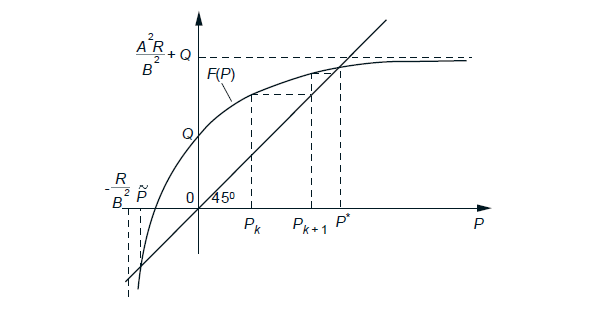
\includegraphics[width=12cm]{Lecture4/Fig1.png}
    \item Gnerally, as $k\to\infty$, the corresponding steady-state controller $\mu^*(x)=Lx$, \\
    where $L=-(B^TKB+R)^{-1}B^TKA$ \\ $L$ is stable in the sense that the matrix $(A+BL)$ of the closed-loop system \\
    $x_{k+1}=(A+BL)x_k+w_k$ satisfies $\lim_{k\to\infty}(A+BL)^k=0$
\end{itemize}

\subsection{Random System Dynamics}
\begin{itemize}
    \item Suppose that $\{A_0,B_0\},...,\{A_{N-1},B_{N-1}\}$ are not known but rather are independent random matrices that are also independent of the $w_k$
    \item $J_k(x_k) = \min_{u_k}\mathbb{E}_{w_k,A_k,B_k}\{ x_k^TQ_kx_k + u_k^TR_ku_k + J_{k+1}(A_kx_k+B_ku_k,w_k) \}$
    \item $L_k = -(R_k+\mathbb{E}\{ B_k^TK_{k+1}B_k \})^{-1} \cdot \mathbb{E}\{ B_k^TK_{k+1}A_k \}$
    \item $K_k=\mathbb{E}\{ A_k^TK_{k+1}A_k \} - \mathbb{E}\{ A_k^TK_{k+1}B_k \} \cdot (R_k+\mathbb{E}\{ B_k^TK_{k+1}B_k \})^{-1}\cdot \mathbb{E}\{ A_kK_{k+1}B_k^T \} + Q_k$
    \item Properties
    \begin{itemize}
        \item Certainty equivalence may not hold.
        \item Riccati equation may not converge to a steady-state.
        \item In simple case, we have $P_{k+1}=\tilde{F}(P_k)$, where \\
        $\tilde{F}(P)=\frac{\mathbb{E}\{ A^2 \}RP}{\mathbb{E}\{B^2\}P+R} + Q + \frac{TP^2}{\mathbb{E}\{B^2\}P+R}$\\
        $T = \mathbb{E}\{A^2\}\mathbb{E}\{B^2\}-(\mathbb{E}\{A\})^2(\mathbb{E}\{B\})^2$
    \end{itemize}
\end{itemize}
\newpage
\subsection{Inventory Control}
\begin{itemize}
    \item State: Inventory level $x_k$
    \item Control: Number of orders $u_k$
    \item Disturbance: Demand $w_k$
    \item Dynamics: $x_{k+1}=x_k+u_k-w_k$
    \item Stage Cost: Ordering cost + maintenance cost (hold cost, penalty cost) 
    \begin{itemize}
        \item $c\cdot u_k + r(x_k+u_k-w_k)$
        \item $r(x_k+u_k-w_k) = h\cdot \max\{0,x_k+u_k-w_k\} + p\cdot \max\{0,-(x_k+u_k-w_k)\}$
    \end{itemize}
    \item Terminal Cost: $J_N(x_N)=0$
    \item Cost-to-go: $J_k(x+k)=\min_{u_k\geq 0}\{ cu_k+\mathbb{E}_{w_k} \{ r(x_k+u_k-w_k) \} + \mathbb{E}_{w_k}\{ J_{k+1}(x_k+u_k-w_k) \} \}$
\end{itemize}